%% COPYRIGHT: Markus Kollmar
%%
%% This is the main escad manual source. We try document-driven-development.
%% Pictures are stored in "figures" directory and
%% tikz-pictures should be build there before build main escad_manual.tex.
%% We use UTF-8 (UNICODE) encoding for this file and lualatex as latex-engine which works well.
%%
%% BUILD WITH LUALATEX AND FILE UTF-8-ENCODED (RECOMMENDED):
%% lualatex escad_manual.tex
%% biber escad_manual.bcf
%% lualatex escad_manual.tex
%% lualatex escad_manual.tex
%%
%% BUILD WITH PDFLATEX:
%%   pdflatex -interaction=nonstopmode escad_manual.tex
%% BUILD WITH PDFLATEX AND SYNCTEX:
%%   pdflatex -synctex=1 -interaction=nonstopmode escad_manual.tex
%% BUILD WITH EXTERNAL-PACKAGE:
%%   pdflatex -synctex=1 -interaction=nonstopmode --shell-escape escad_manual.tex
%% COMPILATION ALTERNATIVE:
%%   latexmk -pdf escad_manual.tex
%%
%% EMACS STUFF:
%%   (set-keyboard-coding-system 'utf-8)
%%   modes: latex-mode, outline-minor-mode
%%   M-x outline-toggle-children
%%   M-x pdf-tools-install
%%   M-x customize apropos TeX-source-correlate-method -> synctex
%%   M-x TeX-source-correlate-mode
%%
%% UNICODE STUFF:
%%   Get font info of point in emacs: C-u C-x =
%%   In shell find a font which supports a unicode (e.g. 1D11E music-violin-key): fc-list :charset=1D11E
%%%%%%%%%%%%%%%%%%%%%%%%%%%%

\documentclass[a4paper, 12pt, openany]{scrbook}
%\usepackage[T1]{fontenc}         % pdflatex only, for lualatex use instead: \usepackage{fontspec}
\usepackage{fontspec}             % lualatex only, not for pdflatex
%\setmainfont{Latin Modern Roman} % lualatex only (optional) with \usepackage{fontspec}
%\setsansfont{Linux Biolinum O}   % lualatex only (optional) with \usepackage{fontspec}
%\setmonofont{Droid Sans Mono}    % lualatex only (optional) with \usepackage{fontspec}
%\usepackage[no-math]{fontspec}
\usepackage{luacode}              % lualatex only
%\usepackage{lmodern,textcomp}    % Euro symbol
%\usepackage[utf8]{inputenc}      % pdflatex only, umlauts (without \"a)
%\usepackage[ngerman]{babel}      % new german rules
\usepackage[UKenglish]{babel}     % english for toc...
\usepackage[paper=a4paper, left=2cm, top=20mm, bottom=15mm, right=15mm, includefoot, foot=\baselineskip, footskip=10mm]{geometry} % borders
%\usepackage[headsepline,footsepline]{scrpage2} % outdated, it is recommended to use scrlayer-scrpage instead.
\usepackage[headsepline]{scrlayer-scrpage} % line at header
\usepackage[bibstyle=authoryear, citestyle=authoryear, backend=biber, parentracker=false]{biblatex} % biblatex loading with biber (newer than bibtex)
\renewcommand*{\nameyeardelim}{\addcomma\space}
\ExecuteBibliographyOptions{
sorting=nyt,  % Sortierung Autor, Titel, Jahr
bibwarn=true, % Probleme mit den Daten, die Backend betreffen anzeigen
%isbn=false,  % show no ISBN
%url=true     % show URL
bibencoding=utf8 % wenn .bib in utf8, sonst ascii
}
\addbibresource{bibliography.bib} %Bibliographie files loading
% \usepackage{longtable}
\usepackage[table]{xcolor}
\usepackage{booktabs}
\usepackage{amsmath}
\usepackage{rotating}
\DeclareMathOperator\sign{sign}
\usepackage{listings}
\usepackage[autostyle]{csquotes}  % Anführungszeichen mit \enquote{Anführungszeichen}
%\usepackage{tikz-timing}[2009/05/15]
%\lstset{basicstyle=\scriptsize}
\lstset{basicstyle=\footnotesize\ttfamily, numbers=left, numberstyle=\tiny\color{blue}, frame=single, firstnumber=1, keywordstyle=\color{blue}}
%\lstset{basicstyle=\small} 
\lstset{literate=%
    {Ö}{{\"O}}1
    {Ä}{{\"A}}1
    {Ü}{{\"U}}1
    {ß}{{\ss}}1
    {ü}{{\"u}}1
    {ä}{{\"a}}1
    {ö}{{\"o}}1
    {~}{{\textasciitilde}}1
    {°}{{\textdegree}}1
}
\usepackage{upgreek} % uppright (mathly correct) pi in math-mode
\usepackage[locale=DE]{siunitx}
\usepackage{amssymb}
%\usepackage{color}  % colored text-background
\usepackage{xcolor}  % Text color
%\usepackage{pdfpages}
\usepackage{tikz}    % graphical drawing
\usepackage{pgfplots}
\usetikzlibrary{matrix, positioning, shapes}
\usetikzlibrary{arrows, automata, shadows.blur, patterns}
%\usepackage{circuitikz}
%\usetikzlibrary{external} % faster compilation, but uses dangerous --shell-escape
%\tikzexternalize[prefix=figures/] % activate and define figures/ as cache folder
\usepackage{index}
\makeindex
\pagestyle{scrheadings}

\clearscrheadings
\clearscrheadfoot
\newcommand{\MyVorname}{Markus}
\newcommand{\MyNachname}{Kollmar}
\newcommand{\EscadVersion}{0.1.0}
\newcommand{\MyTitel}{Manual for ESCAD version \EscadVersion}
\newcommand{\MyDate}{\today}
\ohead{page: \pagemark}
\chead{
\includegraphics[width=0.4cm]{figures/escad_logo_jan2022.pdf}}
\ihead{\MyTitel}
\ofoot{\MyVorname\, \MyNachname}
%\cfoot{}
\ifoot{\MyDate}

\usepackage[pdftex,
            pdfauthor={Markus Kollmar},
            pdftitle={\MyTitel},
            pdfsubject={\MyTitel},
            pdfkeywords={manual},
%            pdfproducer={Latex with hyperref},
%            pdfcreator={pdflatex}
]{hyperref}  % Metadaten in PDF

\author{\MyVorname \quad \MyNachname}
\title{\MyTitel}


\input{kvmacros}

%% command-reference function {cmd-name}{input}{output}{description}:
\newcommand{\escadcmd}[4]{\index{command reference!#1}
  \colorbox{black!20}{\parbox[c][1em]{160mm}{\texttt{#2}}}\\
  \colorbox{green!20}{\parbox[c][1em]{160mm}{\texttt{#3}}}\\#4}

%% shell command-line {cmd-name}{result}:
\newcommand{\shellcmdline}[2]{\\
  \setlength{\fboxsep}{2pt}\colorbox{black!20}{\parbox{\textwidth}{\texttt{user@host:$\sim$/escad\$ \textbf{#1}\\#2}}}\\}

%% escad command-line {cmd-name}{result}:
\newcommand{\escadcmdline}[2]{\\\setlength{\fboxsep}{2pt}\colorbox{black!20}{\parbox{\textwidth}{\texttt{ESCAD> \textbf{#1}\\#2}}}\\}

%% lisp command-line {cmd-name}{result}:
\newcommand{\lispcmdline}[2]{\\\setlength{\fboxsep}{2pt}\colorbox{black!20}{\parbox{\textwidth}{\texttt{> \textbf{#1}\\#2}}}\\}

%%%%%%%%%%%%%%%%%%%%%%%%%%%%%%%%%%%%%%%%%%%%%%%%%%%%%%%%
\begin{document}

\begin{titlepage}
   \begin{center}

     %\vspace*{1cm}
     
     {\huge \MyTitel \ - \MyDate}

     \vspace{0.5cm}

     {\small by:\ \MyVorname\ \MyNachname}

     \vspace{0.5cm}
     
     \begin{tikzpicture}
       \coordinate(front)at(0,0);
       \coordinate(horizon)at(0,.41\paperheight);
       \coordinate(bottom)at(0,-.6\paperheight);
       \coordinate(sky)at(0,.47\paperheight);
       \coordinate(left)at(-.41\paperwidth,0);
       \coordinate(right)at(.41\paperwidth,0);
       \shade[bottom color=white,top color=blue!40!black!50]([yshift=-120mm]horizon-|left)rectangle(sky-|right);
       \node[circle, fill=orange!30, shade, blur shadow={shadow blur steps=5}] (user) at (0,12) {USER};
       \node[circle, fill=green!20, shade, blur shadow={shadow blur steps=5}] (escad) at (0,0) {ESCAD};
       \node[circle, fill=green!20, shade, blur shadow={shadow blur steps=5}] (world) at (-4,7) {WORLD};
       \node[circle, fill=green!20, shade, blur shadow={shadow blur steps=5}] (view) at (3,5) {VIEW};
       %\draw [thin, gray,-latex] (escad) -- (user);
       \draw [gray] (escad) to [out=50,in=195] (user);
       \draw [red] (escad) to [out=-120,in=165] (world);
       \draw [yellow] (escad) to [out=-60,in=20,looseness=2.2] (view);
       \draw [blue!60] (user) to [out=0,in=20,looseness=2.2] (view);
       \draw [green!60] (user) to [out=140,in=100] (world);
       \draw [red!60] (world) to [out=0,in=100] (view);
       \node[anchor=south west] (escad_logo) at (0,-5) {\includegraphics*[scale=5]{figures/escad_logo_jan2022.pdf}};
     \end{tikzpicture}

     
     \vfill
            
      Alles hängt mit allem zusammen. Wir haben nur nicht das ganze Bild...
            
       \vspace{0.8cm}

     \end{center}
\end{titlepage}


%\maketitle
%\pagebreak
%\cleardoublepage
\tableofcontents
%\pagebreak

\chapter{Introduction}
You have choosen interest in a friendly libre software. This software is aimed to be a workhorse for many tasks which are usefull to do with the help of graph-structure. However to be honest this escad version \EscadVersion\ shows that there is still much to develop. So some things may not work as expected or there are silly mistakes around. But i think it is better to regularly update.

Documentation lives like the code! I recommend - and think it is very useful - to \textbf{read this manual}. Because you get a feeling about escad and its terminology. And unlike some manuals, escad tries a documentation-driven development process, which will be explained in the next section. This makes this documentation a up to date view of the current escad and shows you what can be awaited from escad and what not.
\section{Documentation-driven development}\label{sec:ddd}
Documentation-driven development means here (at least we try), at first we define in this manual what we want to develop mostly from the user perspective. Then the feature will be implemented according this documentation. This is an advantage for the user, since he can see what a feature will look like, and documentation is ahead and not behind the actual implementation. The specified features in the manual, align to the mentioned version of escad. If some feature will be in a later version, this should be mentioned by a version notice. Features which are in the software but not documented here, should not be used or rely on, because they may change or are not ready for production yet.
\section{Philosophy}
History tells us about separation. Separation between different professions was and is common. People have different interests and different knowledge. So this seems natural. Is this a problem? No and yes. Nowadays science goes into a direction where \textbf{interdisciplinarity} seems more important. The bounds of our disciplines are drawn by human but it not need to reflect the reality in nature. This seems not a big problem in many cases. But when it comes to documentation or knowledge transfer tasks, this can be a big problem. The tools often do not interact with each other, and if so they often feel not integrated well. This problem increases when different manufacturers have tools which interact not or very bad. Furthermore real problems are mostly system-problems or are increasingly seen as such. Systems are combined of different disciplines. But do the (software) tools support this fact? Some may but many do not. Escad does! Escad allows theoretically to model various disciplines in one software tool!

Living in todays world is getting more and more complex. There are laws made by human which you have to obey. Additionally mother nature has their ever-lasting rules, overwriting all human rules, and which we should obey to keep the environment healthy for future mankind. Thus people may have the need to get information about this \index{complexity}\textbf{complex} system and tools to make this understandable. Escad is not good in some things. In fact it is really not yet a good graph analysis tool (however one could update that functionality). Escad wants to be a (relatively simple) worker which allows combining different domains in one model: get something out of your semantic-graph-model, avoid switching different tools too much, make \LaTeX\ , PDF, 3D models, music or other documents, which would be boring to create by hand. You can additionally also use the \textbf{scripting} facility of escad.
\section{State and screenshoots}
Currently escad is in (wild) development {\fontspec{DejaVu Sans} 😀}. This means there are many ideas which should be developed. Some are just a quick hack to show what is possible and some are more detailed. However but only usable for experts in some areas. Many things are not completed. This is often to just give the idea what should come and is intended to be completed later if the system interacts satisfactorial as a whole.
Basically you can use escad in two ways:
\begin{itemize}
\item Command line entering common-lisp code, here in the editor emacs, see figure~\ref{fig:escad_emacs}.
\item Graphical user interface via web browser, see figure~\ref{fig:escad_gui}.
\end{itemize}
Escad use open technologies and provide a wide variety of different domain tools. And if there is (yet) not the thing you need, you can customize escad with common-lisp code. Escad wants to be kind and helpful to the user. \textbf{Your help is really welcome}: if you want maintain this manual, increase escad features, write expansions, create logo, manage homepage or just send some feedback - all things are kind to start a escad-community.
\begin{figure}[htbp]
  \centering
  \begin{tikzpicture}[node distance=0.6cm and 1cm]
    \node[anchor=south west] (escad_emacs) at (0cm,0cm) {\includegraphics*[scale=0.35]{figures/escad_emacs.png}};
  \end{tikzpicture}
  \caption{escad in emacs (note the appearance may differ from yours).}
  \label{fig:escad_emacs}
\end{figure}
\begin{figure}[htbp]
  \centering
  \begin{tikzpicture}[node distance=0.6cm and 1cm]
    \node[anchor=south west] (escad_web_ui) at (0cm,0cm) {\includegraphics*[scale=0.4]{figures/escad_web_ui.png}};
  \end{tikzpicture}
  \caption{escad via graphical web-user-interface.}
  \label{fig:escad_gui}
\end{figure}
\section{License}
Escad strictly wants to be open source and helpful for many people. It is licensed under the \emph{GNU AFFERO GENERAL PUBLIC LICENSE Version 3, 19 November 2007}. For more information see the file \path{LICENSE} in your escad root-directory.
\section{Installation and starting}
Currently there are no preconfigured packages for convenient installation of escad. However installation should not be to difficult, since escad-development tries to minimize not shipped dependencies.
\subsection{Linux or unix-like systems}
\begin{enumerate}
\item Get the repository from \path{https://github.com/mkollmar/escad} by clone it, or download repository as zip-file and extracting it. The escad executable is at the root folder and is called \path{escad}. If you want make the excecutable yourself (in the case the preinstalled does not work), then you currently need \textbf{sbcl} common-lisp implementation installed with your distribution-package-method. In the root directory of the repository execute \texttt{make executable} and after some while you will get it.
\item Optional: For some PNG/SVG export functionality you need to have/installed \textbf{graphviz} and for PDF exports you need to have/install a \textbf{lualatex} installed with your distribution-package-method.
\item You can now try to run escad (in terminal-mode) within the escad-root-directory. If you want the command line interface mode then type just \texttt{./escad}. If you want use the browser gui then type \texttt{./escad webgui} and enter in your browser \texttt{127.0.0.1:8529/}.
\item Optional: To make initial settings for escad check the config file \path{escad.conf} and edit if necessary. This file will be read and executed at start of escad and contains escad lisp commands, like the one you type in at escad command line.
\end{enumerate}
\subsection{Other}
Sorry, for now other systems are currently not tested, but may be possible to work, since common-lisp is available for wide range of os. However some additional tools may be not available or have different behaviour so that not all things work like under linux. Another way is trying to start linux in a virtual environment, but knowledge is needed. If there is more man power it may be possible to improve that situation.
\section{How it works and terms}
To understand a software-system it is often easier to understand the theory behind. In escad this is quite simple, since it is practical use of graph data structure (in informatically or mathematically means). But simple means just in the basic building blocks, not in the power, since graphs can be quite big and nested. Such \textbf{graphs} consist only of \textbf{symbols} $V$ (vertices, nodes, Knoten) and \textbf{relations} $E$ (edges, Kanten). Mathematically (see also \cite{math:taschenbuchdermathematik}) you can see this in equations~\ref{eq:graph}:
\begin{align}
  \label{eq:graph}
  V & = \{s0, s1, s2, s3\} \notag \\
  E & = \{r0, r1, r2, r3\} = \{(s0, s1), (s1, s2), (s2, s3), (s3, s2)\}
\end{align}
You see in math you would need no name for relations, as it are ordered pairs of symbols. Escad uses names for symbols and relations. This is because relations can have some optional properties (symbols too), which you can acess via the relation-name. As convenience you can let escad give you automatic generated names, in case you do not care of the exact name.
See figure~\ref{fig:overview} about the structure of escad. The three grey blocks are needed for the interaction with the user (commandline or web interface). Thus they are explained not here but will be looked later in detail. In the following sub-chapters the other three parts and their contents are explained in detail.
\begin{figure}[htbp]
  \centering
  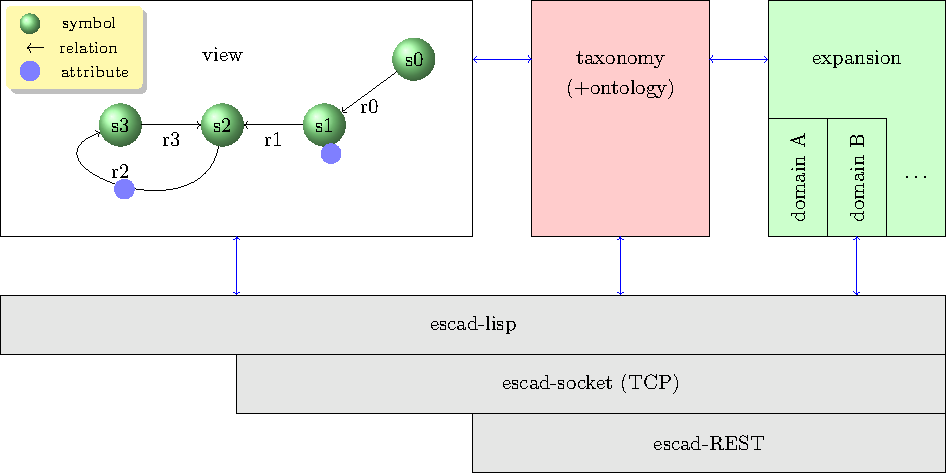
\includegraphics{figures/overview.pdf}
  \caption{Overview of basic escad structure.}
  \label{fig:overview}
\end{figure}
However a short additional security note on the communication blocks: You can communicate with escad through common-lisp. This communication can also piped through a local TCP-connection by the user. Note that for security reasons you should not make such network-communications over the internet, since escad is not encrypted. This is also true for the HTTP connection. It is currently only meant for local network use. However you could use technics like VPN if you want secure transfer through the internet.
\subsection{Symbol}
In many papers a symbol is also called \index{node}node. However escad has the aim to model things into software - a symbol for a concept. Thus a node is a \emph{variable} for something in our thoughts. This symbol can represent a house, a number, a theory, a joke or whatever you want. This shows the great flexibility of escad. In figure~\ref{fig:overview} symbols are circles with names in it (e.g. s0) which you can name however you want, as long it is a unique name in the current graph. In case you do not care, escad can even generate a unique name for you.
\subsection{Relation}
A relation (or in computer science also called \index{edge}edge) creates a relationship or dependency between two symbols. You can specify the meaning of this dependency further. Generally one can divide following classes of dependencies:
\begin{description}
\item[is\_a] can be used to describe/create symbol-hierarchies (also known as hyperonym–hyponym or supertype/superclass $\rightarrow$ subtype/subclass).
\item[has\_a] can be used to define a possessive hierarchy/aggregation (no ownership) between symbols (also known as holonym/whole/entity/container $\rightarrow$ meronym/part/constituent/member).
\item[part\_of] can be used to describe a ownership hierarchy/composition between symbols (also known as meronym/constituent $\rightarrow$ holonym/entity).
\item[member\_of] can be used to describe a containment (also known as meronym/member $\rightarrow$ holonym/container).
\item[instance\_of] can be used to describe a concept-object (also known as token/object $\rightarrow$ type/class).
\end{description}
\subsection{Attribute}
An \index{attribute}attribute in escad is an \emph{optional} specifier of a symbol/relation. There can be a huge discusion whether attributes or whether a symbol and relation should be used instead a symbol-attribute. Attributes can lower the complexity of an graph. On the other hand attributes are implicite relations, perhaps sometimes it is more useful to state explicitely relations (e.g. for graphical purposes). Take your choice and try to keep this choice consistent over your graph. Some attributes merely are parameters which give the symbol or relation additional information, mostly needed in conjunction with expansions (e.g. giving a filename to a file-generation expansion).
\subsection{View}
You can think of the view as a workplace where you can put in symbols and relations, which model an part of the real world. It is called view because it is the current view of a world modelled in your escad session. However like in the real world there are often multiple and different views of the world. Thus you can acess other views through a view-symbol in the standard expansion mentioned later.
\subsection{Taxonomy}
With taxonomy you can create in escad a classification (domain-based) to your symbols and relations by just tagging them. Depending of the taxonomy there may result different (graphical) output or behaviour (functionality) by escad. This may sound clear, since without that a computer can not know what a symbol means just by interpreting its name. But it is merely like a seperator in your folders - you can name and seperate things but you may not do much more. More is possible with the ontology.
\subsection{Ontology}
In semantic-knowledge field you may hear often words like \index{ontology}ontology. Ontology \emph{uses} the taxonomy to capture and represent the meaning of a domain and has rules what is possible with it and what not. Since escad is aimed to be a practical tool, it has some domain specific ontologie-knowledge included. This knowledge is provided by an expansion.
\subsection{Expansion}
Expansions are a collection of \emph{ordinary symbols} for the user with a \emph{additional function}, given by assigning a taxonomy and executed via \emph{activation} of a symbol. Nowadays such easily achivable functionality may be called \index{app}\emph{apps}, who can do various things with your graph. This ranges from graphic output to new generated graph-elements. There are many possibilities and you can even write your own expansion(s). Those programms live in the escad environment and can use the provided feature, even of other expansions. However currently there is only a limited set of expansion, but this could increase in time. Feel free to write a expansion for your domain specific needs.

When we speak of \emph{activation} of a expansion, what does that mean? You as user give a activation command or right-klick on the symbol, then a special function is executed. What special function is that and what does it make? Well in fact it is

Table~\ref{tab:expansion_overview} shows the available expansions included in the current version of escad.
\begin{table}[htbp]
\definecolor{light-gray}{gray}{0.9}
\rowcolors{2}{light-gray}{black!20} % alterniert Farbe der Tabellenzeilen
\centering
\begin{tabular}{|p{2.5cm}|p{6cm}|p{5cm}|p{2cm}|}
  \hline
  \textbf{topic} & \textbf{file} & \textbf{description} & \textbf{since version} \\
%  \hline
%  3D & \path{3d_expansion.lisp} & Generate 3D files. & 0.2 \\
  \hline
  export & \path{export_expansion.lisp} & Export graph to PDF and SVG. & 0.1 \\
%  \hline
%  flow & \path{flow_expansion.lisp} & Automates processes in escad. & 0.1 \\
  \hline
  generation & \path{generator_expansion.lisp} & Generate objects in view. & 0.1 \\
  \hline
  import & \path{import_expansion.lisp} & Import graphviz dot-file in view. & 0.1 \\
%  \hline
%  import & \path{mount_expansion.lisp} & Mount other graphs into view like from a graph database. & 0.1 \\
  \hline
  report & \path{report_expansion.lisp} & Report view to latex and PDF. & 0.1 \\
  \hline
%  standard & \path{standard_expansion.lisp} & Provides common useful concepts like sets, checks or canonizing. & 0.1 \\
%  \hline
\end{tabular}
\caption{Contained expansions in escad and their functionality.}
\label{tab:expansion_overview}
\end{table}
\section{Usage design patterns}
To get things done with escad, there are several tasks you have or want to do. In this section we provide you with common interaction concepts in escad. You also see commands, expansions or taxonomies which are needed for this. But detailed examples you will need in next chapter.
\subsection{Modeling}
Modeling is the way you describe escad your topic/task of interest. This is a very important task. If you model something, look at the given examples in the \path{examples} directory. Use the most approbiate taxonomy. Use expansions to ease your live where possible.
%\subsection{Hiding}
%To view graph networks it is sometimes possible you just want focus on special symbols. Or you want hide symbols which are for configuration tasks (e.g. \emph{\_view} or \emph{\_escad}). This is supported by hiding symbols. Note that the symbols still are active and the expansions still see them. It is only a presentation thing for the user. To hide a symbol create a relation to the \_view symbol with taxonomy \emph{has\_hidden}. So you can read that as \emph{this view has a hidden symbol X}.
%\subsection{Mounting}
%Sometimes you want hide complexity by including another view which even may be on another computer/network or in a graph-database/disk/file. To connect this seperate view with your actual view you can mount symbol(s) of it to your current view. This is like a door where you can hide complexity but if you need more you can open and connect your view with it. Mounting is done with a expansion. After usage you can unmount the seperate view. You would want to do this especially when a complex mounted view is connected through a slow network. Then escad will react slowly too, because it has to fetch/write data to it. Concurent accessing is controlled via a attribute in \emph{\_view} symbol.
\subsection{Exporting}
Saves your view in a non-escad format. This is usefull for use your view in other programms.
\subsection{Importing}
Allows you to get a view stored in a non-escad format.
\subsection{Reporting}
Means to create/process a (new) representation/summary of your view. E.g. your view could be a description of a 3D-modell, and with reporting you could get a 3D-file in X3D-format. A report could also check your view for quality (e.g. if there would occur problems when activate a specific expansion).
\subsection{Generating}
Is used to create new symbols, relations or attributes automatically for you. 
%\subsection{Automating}
%With \emph{flows} automating in escad is possible without to know how to programm in lisp. This also enables live-expansions which periodically activated generate symbols to reflect the state of a continous process.
\chapter{Getting started}\label{cha:gettingstarted}
Here i assume it is easier to get what escad can do for you, by showing escad in work. Note that the output of the following examples may vary a little at your side (becausse of various reasons), but the basic things should be similar.
\section{Tutorial with escad-commandline}
We want now do a short session in escad. After installation go to the escad root directory and start escad by typing in a shell in your terminal:
\shellcmdline{./escad start}{>}
This starts escad REPL (no special arguments given). After loading of common-lisp and escad, you should switch from the common-lisp in the escad namespace:
\lispcmdline{(in-package :escad)}{ESCAD>}
Now you can execute all escad commands directly. To see some possible existing symbols type following escad-command:
\escadcmdline{(ls)}{(``\_escad'' ``\_view'')}\label{ex:ls}\index{command example!ls}
You can read more about this command at page~\pageref{it:ls}. We see two symbols which escad has already created for us. The first symbol can contain settings for our current escad session. The second symbol stands for the current working space we are working. In escad this is called \emph{view} and is just a place where you can work. It can hold graph(s), but does not have to. Escad has two views, you can use (toggle with command \texttt{tv}). But mostly you need just one view.
However we heard that escad has symbols and relations. Lets look at the relations:
\escadcmdline{(lr)}{NIL}\label{ex:lr}\index{command example!lr}
Upps, we get \emph{NIL} which is the lisp way of saying that there is nothing. But that is ok, since we just have not created anything yet. So lets create three symbols:
\escadcmdline{(dolist (name '(``one'' ``two'' nil)) (ns name))}{NIL}\label{ex:ns}\index{command example!ns}
This produces three new symbols, which names we not see because of the \texttt{dolist} nature:
\escadcmdline{(ls)}{(``\_escad'' ``\_view'' ``one'' ``two'' ``s0'')}\index{command example!ls}
The third symbol name \texttt{s0} created escad for us, because we provided \texttt{nil}.
Now lets create a relation:
\escadcmdline{(nr nil ``one'' ``two'')}{``r0''}\label{ex:nr}\index{command example!nr}
Now we got
\escadcmdline{(lr)}{(``r0'')}
Note that you can not insert a new relation or symbol which name already exists.
You now have nearly seen all basic operations in escad. Most functionality can be achieved by this. Instead of learning many new commands, you can use in escad symbols which can also represent actions (e.g. exporting a PDF of your view). But how can you execute such a symbol. This makes the command \emph{as}, which \emph{activates} the given symbol:
\escadcmdline{(as ``s0'')}{(``Documentation text...'')}
You can activate every symbol, but most of them will just print some documentation about themselves, like you have seen in the last command. To get another functionality you have to assign a taxonomy which refers to a expansion. Those expansion is then loaded and executes a defined command (which is defined by the taxonomy).
You can easily add taxonomy to a symbol with add a \emph{property}:
\escadcmdline{(s ``s0'' :taxonomy ``escad.symbol.\_escad.export.pdf'')}{(``s0'')}
If you would activate this smybol now, it would produce a pdf with graphic output of your current view. Because you gave no file-name it would generate some. To give a filename you can add a special attribute-property:
\escadcmdline{(asa ``s0'' '(``filename\_relative'' ``my\_file.pdf''))}{(``my\_file.pdf'')}
Now you should get those pdf-file.
This are the most basic commands you need to know in escad. To get detailed command info use command help:
\escadcmdline{(help-command 'cmd\_name)}{(``Documentation text of cmd\_name...'')}
To get basic help type:
\escadcmdline{(help)}{(``Documentation text...'')}
To load stored views or escad-lisp-scripts (e.g. in the \emph{examples} directory) type:
\escadcmdline{(lov ``mindmap.lisp'')}{(...)}
To list available taxonomies use command \texttt{(lta)}.
\section{Tutorial with graphical browser-interface}
We want now do a web-session in escad. Go to the escad root directory and start escad by typing in a shell in your terminal:
\shellcmdline{./escad start net-http}{>}
This starts escad and a server. With your web-browser you can browse the page which at first time loads a web-client in your browser. After that you can view and edit the graph like in figure~\ref{fig:escad_gui}.
\section{User stories}
To get a fast idea how you should work with escad, please read this section carefully. It gives you general hints how to work, and useful example-patterns to make the theory more clear.
%\subsection{3D (escad version 0.2)}
%Generate 3D-models.
%\subsection{Contact tracing}
%Tool to provide contact tracing, useful by tracking viral deseases (e.g. corona).
%\subsection{Documentation}
%Create (technical) documentation in latex or PDF file-format (reporting).
\subsection{Exporting}
In case you can not do some things in escad yet or other tools may do better, you can export your graph. You can export the view to:
\begin{description}
\item[graphviz-dot] is a file format for graphviz, which is powerful in graphically layout and drawing of graphs. Export with a expansion.
\item[SVG] is a vector graphic-format viewable through most modern webbrowsers.
\item[PDF] Export with a expansion.
%\item[Mindmap] This creates mindmaps in SVG format. Very usefull to view in a browser and to make your graph visible.
\end{description}
%\subsection{Flow}
%Note: this is not working yet, because it is in development!
%A flow is a graph wich models/automates a process. You can use escad to create a process a user should go through (e.g. a question+answer quiz) or a automation which escad should do for you.
\subsection{Importing graphviz dot}
Because interoperability is important in todays heterogenic software world, there should be a way to get graphs from other software.
Graphviz is powerful in graphically drawing of graphs. You can import those graphs with .dot extension. However only basic functionality of dot is currently supported. Import with a expansion.
%\subsection{Learning page (version 0.2)}
%Standalone-HTML-javascript learning page generator Note: this is not working yet, because it is in development! You can generate html-pages with integrated javascript functionality to train some excercises, e.g. language learning. It provides motivational intuitive training pages which you can easily generate without html or javascript knowledge. The user has to do excercises and gets result if anwer is correct or not.
%\subsection{Lessons learned}
%You model e.g. deseases and their dependencies. Then you can try to give symptom(s) and ask for possible cause-tracing.
%\subsection{Music/sound creation (version 0.2)}
%Todo...
%\subsection{Mind-map}
%Model a mind-map for learning support.
\subsection{Modelling}
Modelling semantic graphs is not a easy task. Of course you can make easily symbols and relations, but it heavily depends how you use them. In the past many semantic projects are died or got not very sucessfull used at a wide range. Barry Smith stated some reasons (\url{https://www.youtube.com/watch?v=p0buEjR3t8A}) like silo-syndrome, short-half-life-syndrome and reinvent-the-wheel-syndrome. Nowadays there is a sucessfull example in bioinformatic where to show how genes affect our biology (see BFO-ontology). However even with the best ontology you can have problems, if you not use it properly. To use it you should have a clear knowledge on what the terms mean and how to use.

Such problems may also occur with escad. To improve the situation, escad tries to have many examples for several domains and tasks. The aim is to have enough examples so that you have the possibility to adapt it easily to your needs. I believe it makes more sense to use semantics than to have endless discussions what is the ''correct'' taxonomy/ontology.
%\subsection{Pedigree}
%Todo...
%\subsection{Quiz}
%Todo...
\section{FAQ}
Sometimes questions lead to a fast recognition of a problem or help to understand things better. Not all questions may be frequently asked, but who cares :-)
\subsection{Scope}
\begin{description}
\item[I really do not understand whether escad is for me?] Do you search a nice software to make crazy pictures of your graph in a interactive way? Then you currently may not be right here, just look at something like gephi. Escad is for people who want to work exactly and reproducible with graphs in a more describing manner and in a second step there will be an output (similar like batch processing).
\item[Can i make complex queries like in a graph database?] Perhaps you need a graph database, escad is not a pure graph database. It is a tool, not designed as a speed optimized storage container. However it is planed to have a graph-database connection (e.g. to great arangodb) in order to support persistent huge graphs.
\end{description}
\subsection{Usage}
\begin{description}
\item[Is there a difference in the power of the different escad interfaces?] Yes. The most powerful is currently the command line interface. New commands appear first there. The aim is to keep the functionality equal across the interfaces in a later step. But each interface has it strength, thus it makes sense to use all. Where the commandline has powerful scripting capabilities, the web-interface allows a more intuitive and haptical way to interact with the graph and shows a fast overview.
\item[Why you have choosen common-lisp as the language for escad?] While having some experience with different languages, lisp has one of the clearest syntax for me. The REPL allows interactive rapid prototyping. Lisp is an old but mature language. One can implement easily a domain specific language (DSL) if needed.
\end{description}
\subsection{Development}
\begin{description}
\item[Can i help develop escad?] Of course, very welcome! This currently is a project done in spare free time beneath work. So just contact the developer in github to improve escad together.
\end{description}
\subsection{Other}
\begin{description}
\item[Is there support for other languages as english?]  No not currently. The main author is german, but has spare time to keep manual in german as well. Currently english is choosen to reach a wide international range of people. If you want contribute with translation for your language feel welcome.
\end{description}
\chapter{Reference}
Here you should find the full information to work with escad, such as available commands or interfaces. Also you should get some basic things in order to get the idea in how you can extend escad or help in development.
\section{Commandline LISP-REPL}\label{sec:cmd_line}
The commandline currently provides the full functionality. This means you got a common-lisp REPL with escad-package loaded. This gives you the full power of common-lisp with the ability of the escad-commands to work with a simple graph environment. To get this commandline go to the escad root directory and start escad-commandline by typing in a shell in your terminal:
\shellcmdline{./escad start terminal}{>}
or because terminal-mode is the default you can also type:
\shellcmdline{./escad start}{>}
Without correct command arguments you get a usage message.
Now you can type in escad commands with a namespace-qualifier, in this case the help command (note the output is here ommitted):
\lispcmdline{(escad:help)}{...}
In order to omitting this namespace just type once:
\lispcmdline{(in-package :escad)}{ESCAD>}
Now you can type just (note the output is here ommitted):
\escadcmdline{(help)}{...}

The table~\ref{tab:cmd_abbreviatons} explains used symbols, abbreviations and the data-structures in the reference.
\begin{table}[htbp]
%\definecolor{light-gray}{gray}{0.9}
%\rowcolors{2}{light-gray}{black!20} % alternates color
\centering
\begin{tabular}{lp{6cm}p{6cm}}
  \textbf{PATTERN} & \textbf{DESCRIPTION} & \textbf{EXAMPLE} \\
  \toprule
  ATTR & attribute taxonomy string & \texttt{``escad.attribute.author''} \\
  \midrule
  \textbf{cmd} & command name & \textbf{asa} \\
  \midrule
  (ATTR STRING ...) & attribute taxonomy value list & \texttt{(``escad.attribute.author'' ``Author Name'')} \\
  \midrule
  NIL & common lisp nil means not true/done & \texttt{NIL} \\
  \midrule
  RN & relation name string & \texttt{``r0''} \\
  \midrule
  SN & symbol name string & \texttt{``s0''} \\
  \midrule
  RO & relation object & \texttt{``r0''} \\
  \midrule
  SO & symbol object & \texttt{``s0''} \\
  \midrule
  STRING & string with unspecified or multiple semantic & \texttt{``a message string...''} \\
  \midrule
  VN & view number & \texttt{0} \\
  \midrule
  + & previous content can occur at least once or multiple times & \\
  \midrule
  * & previous content can occur not or multiple times & \\
  \midrule
  ... & previous pattern can be continued & \texttt{(0 1 2 ...)} \\
  \midrule
  () & basic common-lisp list & \texttt{(1 ``Hello'')} \\
  \midrule
  \lbrack\ \rbrack & optional argument(s) & \texttt{(cmd \lbrack\ \rbrack)} \\
  \midrule
  \colorbox{black!20}{function argument} & function argument & \\
  \midrule
  \colorbox{green!20}{function result} & function result, multiple values seperated by comma are possible & \\
  \bottomrule
\end{tabular}
\caption{Explained abbreviations and symbols.}
\label{tab:cmd_abbreviatons}
\end{table}
In general escad provides two flavours of commands: object- or text-based. There is no superior flavour, just use the one which fits your concrete needs the best. This command reference is sorted alphabetically, so the order of commands does not say something about the quality or importance of them.
\begin{description}% \item[$\to$]
\item[\parbox{8.5mm}{ad}] \label{it:ad} \escadcmd{ad}{}{STRING}{<a>nalyze <d>iameter (length of longest path(s)) of current view and returns multiple values: the diameter of longest path(s) and the path(s) itself.}
\item[\parbox{8.5mm}{as}] \label{it:as} \escadcmd{as}{\lbrack\ SN \rbrack}{STRING}{<a>ctivate <s>ymbol in current view.
What happens depends on the taxonomy of the symbol. Many symbols print out a string as their contents.
Symbols which represent expansions will execute the configured function of the expansion.}
\item[\parbox{8.5mm}{asa}] \label{it:asa} \escadcmd{asa}{SN (ATTR STRING ...)+}{SN | NIL}{
<A>dd/edit <s>ymbol <a>ttributes depending of key. NIL if nothing is added.}
\item[\parbox{8.5mm}{gra}] \label{it:gra} \escadcmd{gra}{RN attribute-string}{STRING}{<G>et <r>elation <a>ttributes depending of given attribute-string.}
\item[\parbox{8.5mm}{gsa}] \label{it:gsa} \escadcmd{gsa}{SN attribute-string}{STRING}{<G>et <s>ymbol <a>ttributes depending of given attribute-string.}
\item[\parbox{8.5mm}{help}] \label{it:help} \escadcmd{help}{}{STRING}{Print <help>ful overview of escad, meaning of terms and all available commands.}
\item[\parbox{8.5mm}{lr}] \label{it:lr} \escadcmd{lr}{\lbrack\ :filter :exclude-taxonomy \rbrack}{(RN*)}{<L>ist all <r>elations in current schematic which name match the filter. Additionally exclude relations which match the exclude-taxonomy.}
\item[\parbox{8.5mm}{ls}] \label{it:ls} \escadcmd{ls}{\lbrack\ :filter :exclude-taxonomy \rbrack}{(SN*)}{<L>ist all <s>ymbols in current schematic which name match the filter. Additionally exclude symbols which match the exclude-taxonomy.} See example at page~\pageref{ex:ls} for usage.
\item[\parbox{8.5mm}{nr}] \label{it:nr} \escadcmd{nr}{RN | nil SN SN \lbrack\ :attributes :comment :taxonomy :weight \rbrack}{RN | nil}{Create <n>ew <r>elation with given name and possible additional values in view. If the relation-name already exists do nothing and return nil. Default type is undirected relation. To make a directed or bidirected relation, set the appropriate taxonomy (note that ref\_from and ref\_to are only technical terms meaning you first tie the relation from that symbol to another. it can mean that is directe, but it is not guaranted that the author means that unless he makes that explicit with a relation that declares that).}
\item[\parbox{8.5mm}{ns}] \label{it:ns} \escadcmd{ns}{SN | nil \lbrack\ :attributes :comment :taxonomy :weight \rbrack}{SN | nil}{Create <n>ew <s>ymbol with given name and possible additional values in view. If the symbol-name already exists do nothing and return nil.}
\item[\parbox{8.5mm}{r}] \label{it:r} \escadcmd{r}{RN \lbrack\ :comment :ref\_from :ref\_to :taxonomy :weight \rbrack}{RO | nil}{Get/set <r>elation object.}
\item[\parbox{8.5mm}{s}] \label{it:s} \escadcmd{s}{SN \lbrack\ :comment :taxonomy :weight \rbrack}{SO | nil}{Get/set <s>ymbol object.}
\item[\parbox{8.5mm}{tv}] \label{it:tv} \escadcmd{tv}{}{VN}{<T>oggle <v>iew since escad has two views change from the one to the other and gives back the number of the new view (0 or 1).}
\item[\parbox{8.5mm}{vs}] \label{it:vs} \escadcmd{vs}{}{(VN SC1 RC1 SC2 RC2)}{Gives <v>iew <s>tatus.}
\end{description}
%\section{Emacs with LISP-REPL and view buffer}
%This is currently possible for experienced users via slime-mode in emacs.
%\section{Tk GUI}
%This is in development but currently in sleep, because other user interfaces are prefered.
\section{Library}
To use escad as a library in your common lisp programm, just load \path{package.lisp}.
\section{HTML-webclient}
Take your browser to communicate with escad in a graphical intuitive way.
\section{Included expansions}
Those are the expansions which are included/shipped in this escad-package. Of course there can exist many more not shipped one, but you should check this in escad yourself by exploring the \emph{\_escad} symbol (how this is done you can see in the \ref{cha:gettingstarted}). This is always the most up to date state.
\begin{description}
\item[taxonomy] is the unique name of the expnsion.
\item[in] shows which relations are allowed/make sense to point to the expansion. If there is none, the symbol is meant to stay unique.
\item[out] shows which relations are allowed to point out of the expansion to other symbols/expansions. If there is none, the symbol is meant to stay unique.
\item[attribute] which are allowed/expected/needed.
\item[description] tells what the expansion does.
\end{description}
\subsection{export\_expansion.lisp}
The table~\ref{tab:exp-export-expansion} explains the export expansion.
\newcommand{\tabitem}{~~\llap{\textbullet}~~}
\begin{table}[htbp]
\centering
\begin{tabular}{rp{11cm}}
  \toprule
  \textbf{taxonomy} & \colorbox{black!20}{escad.symbol.\_escad.export.dot} \\
  \textbf{in} & - \\
  \textbf{out} & - \\
  \textbf{attribute} & 1. symbol name \\
                     & 2. [file name] \\
  \textbf{description} & exports view to dot (graphviz) \\
  \midrule
  \textbf{taxonomy} & \colorbox{black!20}{escad.symbol.\_escad.export.pdf} \\
  \textbf{in} & - \\
  \textbf{out} & - \\
  \textbf{attribute} & 1. symbol name \\
                     & 2. [file name] \\
  \textbf{description} & exports view to pdf \\
  \midrule
  \textbf{taxonomy} & \colorbox{black!20}{escad.symbol.\_escad.export.svg} \\
  \textbf{in} & - \\
  \textbf{out} & - \\
  \textbf{attribute} & 1. symbol name \\
                     & 2. [file name] \\
  \textbf{description} & exports view to svg. \\
  \bottomrule
\end{tabular}
\caption{Symbols and relations of export expansion.}
\label{tab:exp-export-expansion}
\end{table}
%\subsection{flow\_expansion.lisp}
%Todo...
\subsection{generator\_expansion.lisp}
Todo...
\subsection{import\_expansion.lisp}
Todo...
\subsection{report\_expansion.lisp}
Todo...
%\subsection{standard\_expansion.lisp}
%Todo...
\chapter{Development}
Everyone is needed and welcome for escad development. If you are a graphical designer, you are got in documenting or you like to program in lisp or you are interested in web-programming - all is required in escad. :-)
The project is managed with the famous source-code management tool \emph{git} (also known as used in the linux kernel development). The repository is hosted under \url{https://github.com/mkollmar/escad}.

A \emph{Makefile} contains the basic task to generate the code or documentation. So it may be a good choice to look into it in order to get a basic idea how all works. Nevertheless the next sections contain how the development process is (currently) structured. It follows a brief overview over the directory structure and a explanation what it contains (or should contain in the future). The last section provides information in how to program a expansion and the interface
\section{Development process and quality}
As mentioned at page~\pageref{sec:ddd} escads development follows the documentation-driven approach.
All follows this process in short:
\begin{enumerate}
\item Set version according to semantic versioning \parencite{web:semver}
\item Update/create documentation (this manual)
\item Develop along documentation
\item Test
\item Tag version and deliver it.
\end{enumerate}
A note to tests as it seems to become one big factor of good code quality. Surely test are a good method to check well defined interfaces. So here we implement tests too. However because at the early development stage of escad and limited man power, tests will not take as much room as there could be. Since interfaces may change often we will concentrate at often used functions and in more stable versions of escad the tests should be increased.
\section{Directory and files}
The directory structure and some basic files of the repository will be explained in this section. In the root of the repository there are following files with their purpose:
\begin{description}
\item[Makefile] contains the instructions for the \emph{make} programm and controls the most part of escad development process (generating documentation, binary or other things). Just enter \texttt{make} in the command line to see available options.
\item[LICENSE] holds the license to which terms you have to use escad.
\item[README.md] is mostly for github where escad is hosted and contains shor overview about the project.
\end{description}
\subsection{doc/}
Contains the escad documentation for user and developer. Currently this is mainly this manual written in \emph{latex}. But in future a unix man-page, more examples or online documentation would be great, too.
\subsection{lisp/}
\path{lisp/} contains the escad-lisp files with the implementation.
\subsection{lisp/expansion/}
\path{lisp/} contains all escad-expansions which are available.
\subsection{lisp/examples/}
\path{examples} contains examples which can be loaded in escad. But note that currently not all may work yet, they are more a print what a future interface should look like.
\subsection{misc/}
Contains miscellaneous things which have no other place where it fits.
\subsection{test/*}
Here there are unit tests, which execution may be controlled with make.
\subsection{web-gui/*}
The web based graphical user interface (gui) things, which are executed in the web-browser, live here.
\section{Programming your own expansion}
Writing escad expansions is not difficult. Go through following steps carefully and you will have a good basis for writing your own. The code in listing~\ref{listing:exp_minimal} shows a minimal expansion and the listing~\ref{listing:exp_tax} shows the entry in a taxonomy file.
\begin{lstlisting}[caption={Minimal expansion code.}, language=Lisp, morekeywords={in-package, use}, label=listing:exp_minimal]
(in-package "COMMON-LISP-USER")
(defpackage :de.markus-herbert-kollmar.escad.expansion.hello_world
  (:use :common-lisp :escad)
  (:export :my-function)
  (:documentation "This is my expansion which does nothing usefull."))
(in-package :de.markus-herbert-kollmar.escad.expansion.hello_world)
(defun my-function (symbol-name-string)
"This function will be executed by calling this expansion.")
\end{lstlisting}
\begin{lstlisting}[caption={Entry in a taxonomy-file.}, language=Lisp, morekeywords={}, label=listing:exp_tax]
(:taxonomy "escad.symbol.hello_world" :doc "[E] Hello world."
:expansion "hello_world_expansion.lisp"
:package :de.markus-herbert-kollmar.escad.hello_world
:function "my_function"
:license "GNU GPL 3")
\end{lstlisting}
Following things you should keep in mind:
\begin{itemize}
\item Choose namespace.
\item Provide documentation within your expansion.
\item Provide at least one function which can be called with the symbol-name-string as first argument und some possible further arguments.
\item Provide a taxonomy file with your expansion declaration or request that your expansion will be taken into the default escad-taxonomy.
\end{itemize}
You are wellcome if you want include your expansion in this escad distribution.

\clearpage % newpage allows to let appear figures after creating new page.
%\newpage

%%%%%%%%%%%%%%%%%%%%%%%%%%% BIBLIOGRAPHY
% \bibliographystyle{plain}
\printindex
%\bibliographystyle{alpha}   % with bibtex
%\bibliography{bibliography} % with bibtex

\setlength{\bibitemsep}{1em} % Abstand zwischen Eintraegen im Literaturverzeichnis
%\pagenumbering{Roman} %% Seitennummerierung auf römisch
%\setcounter{page}{\value{mysavedromanpagecount}}
\printbibliography[heading=bibintoc] % with biber

%% Abkuerzungen:
% \chapter*{Abkürzungsverzeichnis}
% \begin{acronym}[FLOSS]
%   % \acro{Kürzel}[Kurzform]{Langform}
%   \acro{acid}[ACID]{Atomicity Consistency Isolation Durability}
%   \acro{api}[API]{Application Programming Interface}
%   \acro{aql}[AQL]{ArangoDB Query Language}
%   \acro{cad}[CAD]{Computer Aided Design}
%   \acro{cae}[CAE]{Computer Aided Engineering}
%   \acro{css}[CSS]{Cascading Style Sheets}
%   \acro{db}[DB]{Datenbank}
%   \acro{dbs}[DBS]{Datenbanksystem}
%   \acro{dbms}[DBMS]{Datenbankmanagementsystem}
%   \acro{dfs}[DFS]{Depth First Search}
%   \acro{ekp}[EKP]{Entwicklungs- und Konstruktionsprozess}
%   \acro{erp}[ERP]{Enterprise Resources Planning}
%   \acro{floss}[FLOSS]{Free/Libre Open Source Software}
%   \acro{html}[HTML]{Hypertext Markup Language}
%   \acro{http}[HTTP]{Hypertext Transfer Protocol}
%   \acro{json}[JSON]{JavaScript Object Notation}
%   \acro{lpg}[LPG]{Labeled Property Graph}
%   \acro{nosql}[NOSQL]{Not Only SQL}
%   \acro{pdm}[PDM]{Produktdatenmanagement}
%   \acro{pep}[PEP]{Produktentstehungsprozesses}
%   \acro{rdf}[RDF]{Resource Description Framework}
%   \acro{rest}[REST]{Representational State Transfer}
%   \acro{sql}[SQL]{Structured Query Language}
%   \acro{uml}[UML]{Unified Modeling Language}
%   \acro{url}[URL]{Uniform Resource Locator}
%   \acro{xml}[XML]{Extensible Markup Language}
%   % \acroplural{Kuerzel}[Kurzform des Plurals]{Langform des Plurals}
% \end{acronym}
% \addcontentsline{toc}{chapter}{Abkürzungsverzeichnis} % Abkürzungsverzeichnis in Inhaltsverzeichnis auflisten

\newpage
\listoffigures{} %% Abbildungsverzeichnis
\addcontentsline{toc}{chapter}{\listfigurename} % Figurenverzeichnis in Inhaltsverzeichnis auflisten
\newpage
\listoftables{} %% Tabellenverzeichnis
\addcontentsline{toc}{chapter}{\listtablename} % Tabellenverzeichnis in Inhaltsverzeichnis auflisten




\end{document}
